\documentclass[11pt]{article}                     
\usepackage{graphicx}
\usepackage[section]{placeins}
\usepackage{color}
\usepackage{lineno}
\linenumbers
%
% \usepackage{mathptmx}      % use Times fonts if available on your TeX system
%
% insert here the call for the packages your document requires
%\usepackage{latexsym}
% etc.
%
% please place your own definitions here and don't use \def but
% \newcommand{}{}
%
% Insert the name of "your journal" with
% \journalname{myjournal}
%
\begin{document}

\title{A game-theory modeling approach to utility
  and strength of interactions dynamics in biomedical research social networks}
%\title{Two games modeling approach to collaboration dynamics in biomedical
%research social networks}

%\thanks{Grants or other notes
%about the article that should go on the front page should be
%placed here. General acknowledgments should be placed at the end of the article.}

%\subtitle{Do you have a subtitle?\\ If so, write it here}

%\titlerunning{Fitness \& trust in biomedical research networks}     

%\titlerunning{Short form of title}        % if too long for running head

\author{J. Mario Siqueiros-Garc\'ia         \and      Rodrigo Garc\'ia-Herrera \and         Enrique Hern\'andez-Lemus \and
        Sergio A. Alcal\'a-Corona  %etc.
}

%\authorrunning{Short form of author list} % if too long for running head

%% \institute{J. Mario Siqueiros-Garc\'ia \at
%%   IIMAS-UNAM. Circuito Escolar 3000, Cd Universitaria, Coyoacán, Ciudad de México, D.F. \\
%%               Tel.: +123-45-678910\\
%%               Fax: +123-45-678910\\
%%               \email{jmario.siqueiros@iimas.unam.mx}           %  \\
%% %             \emph{Present address:} of F. Author  %  if needed
%%               \and
%%               Rodrigo Garc\'ia-Herrera,\\ Enrique Hern\'andez-Lemus, \\ Sergio A. Alcal\'a-Corona \at
%%               National Institute of Genomic Medicine\\
%%               Perif\'erico Sur 4809, Arenal Tepepan, Tlalpan, 14610, \\
%%               Ciudad de M\'exico, D.F., M\'exico  
%%            %% S. Author \at
%%            %%    second address
%% }

\date{\today}
% The correct dates will be entered by the editor


\maketitle

\begin{abstract}

  What would happen if researchers in a community were given the same
  amount of resources and then set free to interact among each other?
  How would these resources be distributed in the population after
  many interactions? The final result may be determined by the
  researchers' social and political power, an by their
  prestige. Nevertheless, all these attributes depend, to a certain
  degree, on the research collaboration social network in which
  scientists are embedded. Here we develop a model based on the
  Prisoner's Dilemma implemented on a collaboration network. With this
  model we explore the distribution of resources and the dynamics of
  the strengthening or weakening of collaboration connections among
  partners, as scientists cooperate or defect in order to gain access
  to others' resources. The network is based on data about projects
  that were awarded with a grant. In this sense, we assume that
  resources are funds, equipment and time. We define Fitness as how
  much access a researcher has to the resources of his collegues.  We
  tested our simulation on the real biomedical research network and
  compared the results with an Erd\"{o}s-Reny\'i, a Watts-Strogatz
  small-world and Barab\'asi-Albert topologies. Different topologies
  display different fitness and connections strength
  distributions. Moreover, the distribution of fitness and connections
  strength in the researchers network is similar to that of
  Barab\'asi-Albert and Watts-Strogatz topologies, respectively. We
  believe that fitness distribution in the researchers network
  suggests that there are socio-cultural mechanisms governing the
  network that produce an asymmetric distribution of resources. The
  high distribution of strong connections might reflect some sort of
  subordination among researchers by which they are morally obliged to
  cooperate by the same socio-cultural mechanisms. The range around
  the threshold that regulates the decision to cooperate or defect
  according to the agent's historical balance between utility and
  strength of collaborative relationships and carrying capacity of the
  system is small, suggesting that there is a region in which a phase
  transition takes place from a population of cooperators to a
  population of defectors. Simulations like this may help to develop
  science policies to promote fair distribution of resources.


\end{abstract}

\section{Introduction}
\label{intro}

\textbf{Notes:}

\begin{itemize}

%% \item In this paper there are two games played simultaneously: One for
%% maximazing individual utility; the second for maximazing the connection
%% strength. We are interested in how they affect eachother in the context of a
%% network of collaboration.


\item We change utility for fitness. Utility seems a better concept in order to
  reflect players' preferences.  

%% \item In the context of our paper, utility represents
%%   the preference for having access to the resources of others. Maximazing
%%   utility means that the player is increasing its access to the resources of
%%   other players.  Utility function is just the sum of the payoffs of playing
%%   with its neighbors. As for the payoff matrix, the best strategy for a player
%%   is to defect. Any other option will not be an optimal payoff. The opossing
%%   force is in the other game. The game for maximazing the strength of the
%%   connection among players. In this case defecting or cooperating? is the best
%%   strategy as it pays the most when coordinating regardeless they both cooperate
%%   or defect, this is because when both cooperate the interaction gets a positive
%%   payoff, when both defect, the interaction doesn't get affected; but if they
%%   anti-coordinate, then the interaction looses. In this sense, this might be a
%%   game were there are multiple (i.e., 2 points or strategies) equilibria. It
%%   seems that there is no single dominant strategy.}\\
  

\item Choosing a strategy depends on the balance $\eta'$ equation --look at page
  9. This
  equation states that the probability of an agent to cooperate increases as: a)
  its utility increases --as it moves away from 0, or; b) The strength of the
  connection with its peers increases --as it moves away from 0, or; c) both
  increases.

  $\eta_i = \frac{\langle f_i \rangle + \langle w_{ij} \rangle _j}{2}$\\

\item{En la pagina 9 decimos que ``In order for the agent to choose to cooperate
  or defect, a degree of willingness to cooperate is assigned to each agent.'' No estoy
  seguro que ``degree of willingness to cooperate'' sea la mejor manera de
  decirlo, mi duda está en la palabra ``degree'', por lo que cambi\'e la
  oraci\'on a: The probability for an agent to cooperate or defect depends on a
number that referes to a historical balance between average utility and the average strength of
the connections with its neigbors. }

  
\end{itemize}

Collaboration has become a cornerstone in biomedical research today.
In contrast to physics which has a long history and experience in
collaborative projects, biology is only recently becoming an evermore
collaborative discipline\cite{Vermeulen2013}. Biology has an
interesting record in such matters because scientific collaboration
means something different to different branches of biology: molecular
biology has traditionally been a research activity of small
laboratories\cite{KnorrCetina1999,Strasser2006}, whereas in natural
history there has been data and samples exchange since the $XVII^{th}$
century\cite{Muller2012,Strasser2012}. Despite the differences in
culture and practices, the Human Genome Project made collaboration a
central feature of biology.\\


Nowadays it is widely acknowledged that collaboration takes many
forms, from sharing of biological samples and biobanking to
international groups in charge of helping research communities to
harmonize and share their data. Sharing resources such as equipment,
funds, and time is critical; building trust among scientists is
fundamental. Also, resources are mobilized in order to create strategic alliances.\\


The analysis of cooperation in scientific research has been the subject of a
number of studies
\cite{Vermeulen2013,Newman2001,Newman2004,Elango2012,HernandezLemus2013,Strasser2006,Strasser2012}. This
is not surprising since cooperation and competition are quite important in
today's academic success. How does collaboration happen within a competitive
academic environment and what kind of payoff is present in these settings were
questions considered recently by Wardil and Hauert \cite{Wardil2015} in the
context of cooperation in multi-authored publications. Also, the role of game
theory over complex scientific information and collaboration networks has
attracted attention, mainly focusing on how long-term strategies may shape
different scenarios for Nash equilibria \cite{hanauske2012}. Prisoner's Dilemma
has been used in the study of impact factor and collaboration
\cite{Hara_etal_2002,Lieberman_etal_2005}. \\  

Even with all these research efforts, cooperation in the context of
scientific collaboration is still loosely defined and the long term
dynamics of academic cooperation (and its consequences) are yet to be
fully elucidated. Furthermore, to our current knowledge, there has
been no use of game theory and complex network analysis for
understanding how the topology of scientific collaboration networks
affects access to resources among individuals present in the network
\footnote{For an account of scientific collaboration and definitions,
  please refer to \cite{Sonnenwald2007}.}. Our work aims to contribute
to our current understanding on the matter, specially when agents have
to maximize their access to resources while taking care of their collaboration links.\\


  %% nevertheless
  %% and to a certain degree, the idea behind the model is ethnographically
  %% inspired\footnote{For a mixed methodology approach to scientific
  %%   collaboration refer to Hara et al., 2002 \cite{Hara_etal_2002}.}. In
  %% previous work we observed that members of biomedical research groups interact
  %% strongly with each other but interactions between groups are only
  %% superficial. Our ethnographic work also allowed us to see how difficult is for
  %% Principal Investigators to collaborate with peer groups that are considered
  %% somehow equal in terms of different criteria such a productivity or power. On
  %% the other hand, collaboration may be easier with groups that are far beyond in
  %% some of these terms. This seems to be so because when dealing with a smaller
  %% group, the stronger one can establish conditions of collaboration; when the
  %% group is weaker, there might be a lot to win. For example, this latter
  %% situation can be seen when local groups collaborate with research groups form
  %% overseas, specially from the US.}\\




%% {\color{red}The question behind our model rests on three premises: Scientist
%%   have self-interests and may act seeking their own interests; Scientific
%%   collaboration needs researchers to cooperate and build relationships that can
%%   last; Scientific collaboration networks have a particular topology. Under such
%%   context, if the same amount of resources were given to every researcher at the
%%   same point in time, how would the access to resources be distributed, in the
%%   long run, in a population of interacting researchers that seek to improve
%%   their profits but at the same time have to invest in building trustworthy
%%   relationships with their colleagues?}
%%\\

  %% Seen from a different point of view, how would trust be
  %% distributed in a population of researchers that are mainly interested in
  %% improving their profits, even when acting selfishly always could have a
  %% negative impact on that primary objective?}\\  

 {\color{red}In this article we explore the network effect on the distribution
   of players having access to certain amount of resources from other players in the
   network and the distribution of the strength of connections among
   them. Particularly, we implemented two games played simultaneously: 
   one for maximazing individual utility based on the iterated Prisoner's
   Dilemma; the other, a coordination game for maximazing the connection strength between
   players. We are interested in how they affect each other in 
   the context of a network of scientific collaboration under the idea that while
   researchers are interested in maximazing their utilities, they also know that
   it is important to invest in building collaborative relationships. These two
   behaviors are explored in a biomedical research community of M\'exico.}\\    

{\color{red}In the context of our paper, utility represents
  the preference for having access to the resources of others. Maximazing
  utility means that the player is increasing its access to the resources of
  other players. The value of the Utility function for a player is the sum of the payoffs of playing
  with his neighbors. The opossing force comes from the other concurrent game: players
  trying to maximize the strength of their connections to other players. In the coordinating game
  the best strategy is to adopt the same strategy as the other player, as it pays the most
  regardless of cooperation or defection in the utility game. When
  both cooperate the interaction gets a positive payoff, when both defect, the
  interaction doesn't get affected; but if they anti-coordinate, then the
  interaction looses. Finally, cooperation is a central feature of scientific work.
  For our biomedical network, cooperation can be thought of
  as sharing resources such as time, students, equipment, even money. Examples of defection
  to a cooperator are ghost authorship or
  prestige authorship.

  % este ejemplo de defection no es nada claro:
  %
  % Another example may be a working strategy in which some
  % members of a team do the work at certain moment, and then another part 
  % does its part in some other moment in the future --some sort of
  % reciprocity.

}


The manuscript is structured in five sections. First we describe
\textit{FOSISS}, the main program for grants destined to biomedical applied
research in M\'exico. This is the source of the
database from which we created the researchers collaboration network. Next we
describe our model
and the different network topologies on which we explored it.
We then present our results and discuss them briefly. In the last section
we draw some final remarks and conclusions.


%Our main objective is to achieve a better understanding of the role of network
%topology on scientific collaborative social dynamics. The dynamics of the
%system are explored following the distribution of utility -as a proxy for
%resources- and trust as agents on the network play the Prisoner's Dilemma while
%constrained by trust with their neighbors.\\


%% In order to explore these questions we implemented a game theory simulation on a
%% real social network of biomedical researchers from M\'exico. Game theoretical
%% approaches to cooperation have – of course– been studied for decades. Taking
%% into account the nature of social interaction among players by means of an
%% underlying social network is also an explored topic. Some 10 years ago, Lo and
%% colleagues \cite{Lo2004} formulated a minority game model to connected
%% population within a network and studied the role of connectivity on such
%% games. Later on, Buesser and Tomassini \cite{Buesser2012} studied the dynamics
%% of cooperation for players located on a spatially embedded network in order to
%% categorize the effect that different interaction structures may have in
%% maintaining cooperation (or defection) domains.\\


%% The impact that network topology may have in the robustness of cooperation was
%% investigated in numerical experiments and simulations \cite{Ichinose2013}
%% revealing that clusters of cooperating agents become robust by increasing the
%% number of links to cooperators, with the possible implication that a large
%% number of individuals is required to maintain global cooperation patterns.\\


%% Regarding possible strategies to improve cooperation patterns, several mechanisms such as inequity aversion
%% \cite{Ahmed2014}, social imitation and strategic choice \cite{Vilone2014} have been explored. Inequity aversion is the
%% condition in which individuals care about payoff equality in the outcomes. A kind of moral memory in past outcomes
%% implies that inequity aversion promotes cooperation \cite{Ahmed2014}. Social imitation contrasts with strategic choices
%% in such a way that social influence models may impact on background rationality in decision making. This balance may be
%% behind moody conditional cooperation within a social environment \cite{Vilone2014}.\\


%% The analysis of cooperation in scientific research has been also the subject of a number of studies. This is not
%% surprising since cooperation and competitionare quite important in today’s academic success. How do collaboration 
%% happens within a competitive academic environment and what kind of payoff
%% is present in these settings were questions considered recently by Wardil and
%% Hauert \cite{Wardil2015} in the context of cooperation in multi-authored
%% publications. Also, the role of game theory over complex scientific information 
%% and collaboration networks has attracted attention, mainly focusing on how
%% long-term strategies may shape different scenarios for Nash equilibria \cite{hanauske2012}. \\ 

%% In spite of all these research efforts, cooperation in the context of scientific
%% collaboration is still loosely defined and the long time dynamics of academic
%% cooperation (and its consequences) are yet to be fully elucidated. Furhtermore,
%% to our current knowledge, we are not aware of any work on how the topology of
%% scientific collaboration networks affects the differences of access among
%% individuals to resources present on the network \footnote{For
%%   an account of scientific collaboration and definitions, please refer to
%%   \cite{Sonnenwald2007}.}. In this context our work aims to contribute to
%% further our current understanding on the matter.\\  

%% As has been pointed by others, social research on scientific
%% collaboration is mostly about physics and space research\cite{Vermeulen2013}.
%% Collaboration in biology has been studied to a lesser degree
%% \cite{Newman2001,Newman2004,Elango2012,HernandezLemus2013,Strasser2006,Strasser2012}. The
%% use of game theory, and specifically the Prsioner's Dilemma to understand social
%% dynamics in scientific collaboration can be found at 
%% \cite{Hara_etal_2002,Lieberman_etal_2005}.\\



%% The manuscript is structured in five sections. The following describes \textit{FOSISS}, the main program for grants
%% destined for biomedical applied research in M\'exico. This description is important because that is the source of our
%% database for creating the researchers collaboration network. Next we describe our model, and then, in the following
%% section we introduce the different network topologies on which we explored the model. In the fourth section we present
%% our results and discuss them briefly. In the fifth section we draw some final remarks and conclusions.  


\section{Biomedical research: CONACyT and FOSISS}
\label{sec:1}

CONACyT (National Council of Science and Technology) is the Mexican government
entity in charge of promoting the development of science and 
technology.
Among CONACyT's functions are to develop science and technology
policies according to national needs and demands, to advise the different
instances of government on scientific and technological topics, to promote the
creation of research networks among the scientific community, to grant
scholarships for masters and doctoral studies, and to manage different trusts 
intended to fund individuals and groups for scientific and
technological research.\\

In the year 2002 CONACyT, along with other government agencies and
entities, created sectoral funds
to cover and equally
promote research capacities of different areas such as energy, agriculture
and health. Technological innovation is fostered by the generation of human resources
and by helping research groups to consolidate. It is expected that the
knowledge generated under the sponsorship of these funds
will be the product of applied research that attends national public
needs, and promotes economic growth.\\

\emph{FOSISS} or Sectoral Fund for Health and Social Security Research
(\emph{Fondo Sectorial en Investigaci\'on en Salud y Seguridad Social}) is one of
such funds. FOSISS is constituted by CONACyT, SSA, IMSS and ISSSTE,\footnote{SSA
  is the acronym for Secretariat of Health \emph{Secretar\'ia de Salud}; IMSS is
  the acronym for Social Security Mexican Institute (\emph{Instituto Mexicano
    del Seguro Social}); ISSSTE stands for Institute for Social Security and
  Services for State Workers (\emph{Instituto de Seguridad y Servicios Sociales
    de los Trabajadores del Estado})} being all of them the major public health
providers and research institutions in the country. Every year CONACyT opens a
call for funds limited to a set of health research areas previously defined by a
group of experts. Such areas range from public health issues to chronic and
degenerative diseases.\\  

Eligibility is open to public and private health research sectors,
however most applicants are public universities and research
institutions. From 2002 through 2013, there were 91 institutions funded that
comprised 4988 researchers.\\ 

From these data some important considerations should be made clear. The
population represented in the data include principal investigators (PIs),
associate researchers, postdoctoral associates, postgraduate and undergraduate
students.
% wut? which information is not specified? which is pi and which is undergrad is not specified?
Unfortunately, this information is not specified in the
database. Still, this is something we acknowledge and it's important because
researchers in our network are under different circumstances and we know
that this diversity has a real impact on the structure and eventually on the
dynamics of the network, as well as on the results of our model.\\  

Our database includes the
name of the project, the year it was approved for funding and the research area
to which it was assigned. It specifies the names of PIs or the people 
responsible for the project and the names of collaborators.
Researchers can be PIs in one project and collaborators on a different project. The institutional
affiliation of all participants is included. Through this affiliation
we know the principal institution
behind every project.\\ 

Even though curation and analysis work of the database is still ongoing, some
relevant facts about the biomedical research can be said. Over the period of 12
years, 32 general research areas have been defined, the three most funded
research areas are \emph{chronic and degenerative diseases}, \emph{malignant
  neoplasms}, and \emph{infectious and parasitic diseases}. The least funded
area is \emph{Ethics and medicine}. The area with the most researchers is
\emph{malignant neoplasms}. Other areas of relevance for M\'exico are
\emph{diseases related to poverty} and \emph{Health and vulnerable groups}. \\  

From the institutions that have participated in a protocol funded by FOSISS,
less than one fifth have been responsible for a project and more than 95\% of
them are Mexican, public institutions. There is also an important presence of
foreign institutions as collaborators, most of them from the United States,
though institutions from the UK, France, Spain, Netherlands, Colombia and Cuba
are also in the database.\\ 

Besides the characteristics of the population there are some other boundary
conditions that play an important role on the network topology and dynamics,
that motivated the development of our model. Biomedical research in M\'exico
constitutes a vibrant community and collaboration is part of everyday
work. However, M\'exico does not have public biobanks for research purposes
(which are specially relevant for research in genomics, for example), there is
no regulation on the access to biological samples such as tissue, cells, DNA,
RNA, etc.\footnote{Regulation exists regarding researcher-subject relations
  based on legal and ethical grounds. Also, all projects need to be approved by
  the Ethics Committee and IRB.} Something similar happens with data. There have
been some attempts to create open data repositories for biomedical research, but
they have not been established yet. Regulation on these subjects is still
missing. Finally, technology (e.g., PCR, sequencing and expression profiling
technology) is in the domain of the institutions with the highest research
profiles and sometimes PIs see technology as a personal good.\\  

From our ethnographic work to date, we have been able to see that
biological samples, data and technology can become instruments for negotiating
collaboration. For example, among people involved in research projects, there
are researchers that do not have direct access to samples, simply because their
institution does not offer clinical services. Many of them are non medical
doctors but chemists, biologists, physicists, and mathematicians. There is
another group of researchers that are placed on hospitals who are able to do
research and have access to biological samples from their own patients. It seems
that this group is the most privileged one, and the least pressured to establish
collaboration at whatever cost. Finally, there is one more group formed by those
who work as clinicians at small hospitals with no research infrastructure
whatsoever. This group may have an interest in research and the way for them to
become part of a project and be listed as authors in scientific papers is by
giving researchers who do not have access to biological samples access to
patients.\\

Due to these differences in the access to resources, researchers in
general are compelled to build strategic alliances through which samples, data,
technology and authorship, among other assets, become part of a constant flow through
the network. Social and political capital, as well as concentrations of
resources become fundamental tools for establishing fruitful collaborations. 

\section{Methodology}
\label{sec:2}
%% In this work we developed a model in order to have a better understanding of the
%% distribution of utility and trust in real networks of biomedical research
%% collaboration under certain social constraints  or topological properties.\\  

Our model is based on the iterated version of the Prisoner's Dilemma (PD) and a
coordination game instantiated on
networks. Implementing games on networks is not new and it's an active area of
research aimed to understand the evolution of cooperation in networks populated
by selfish agents \cite{Szabo2007,Nowak1992,Nowak2006,Santos2005,Santos2006}. In many network models
on which some of game theory games are simulated, agents' decision to cooperate
or defect depend on a specific strategy, such as the well known
\textit{tit-for-tat} \cite{Axelrod2006,Nowak2011}. In some other cases, agents
can modify the weight of the interactions with their neighbors
\cite{Santos2006}. From a different perspective others have explored the effect
of different topologies on the emergence of cooperation
\cite{Santos2005,Hauert2004}. {\color{red}In our case, an agent's decision to cooperate or
defect is an outcome that depends on a balance between
utilities and the current strength of its collaboration relationships. Such
balance reflects the overall success or failure of its strategies}. We
study the behavior of the system under different topologies, including a
real-world network.\\  
  

In our model, agents are embedded in a network with varying number of
neighbors. Following the traditional PD game, the strategy chosen by an agent
and the strategy chosen by its neighbors will produce a pay-off. Pay-off follows
the traditional PD rule: $T > R > P > S$. $T$ is for temptation to defect. It is the highest
pay-off and it takes place when the player defects and the other cooperates. $R$
is for reward for when both players cooperate. $P$ is the punishment for when
both players defect. And $S$ is for suckers pay-off, the worst outcome that
takes place when the player cooperates but its neighbor defects. Utility is a
property of agents in which pay-off is accumulated.\\   

{\bf PD utility pay-off matrix}\\

\begin{tabular}{| l | l | l |}
\hline
          & \bf{Cooperate} & \bf{Defect} \\ \hline
\bf{Cooperate} &  $R,R$      &  $S,T$   \\ \hline
\bf{Defect}    &  $T,S$      &  $P,P$   \\ \hline

\end{tabular}\\ \\

The strength of the connection, represented by $w$, is a property of the link between two agents and
gets updated according to an $A_{ij}$ matrix of a coordination game. In the $w$ matrix, the highest value
goes to an edge when both agents cooperate, getting an $R$ for reward, if one of
them defects, the connection gets weaker getting $P$ for the collaborative
connection being punished. If both agents defect, the value $w$ doesn't change,
which means that agents didn't interact or that the interaction gets nullified
$N$. In this game, the best action for any agent is to coordinate with its
neighbor, either beacuse it wins or it doesn't loose. \\ 

{\bf $w$ pay-off matrix}\\

\begin{tabular}{| l | l | l |}
\hline
          & \bf{Cooperate} & \bf{Defect} \\ \hline
\bf{Cooperate} &  $R$      &  $P$   \\ \hline
\bf{Defect}    &  $P$      &  $N$   \\ \hline

\end{tabular}\\ \\


After each game, the agent adds-up utility ($u$), which is the sum of the
pay-offs following the PD matrix. A pair of neighbors will add-up to the strength of
their connection ($w_{ji}$) as they coordinate or anti-coordinate, being $w$
also cumulative. We measure global utility and connection strength for the whole
network. Global utility $U$ is the sum of all individual utilities and global
strength of connections or $W$ is the sum of every pair of agents' links
$w$. Metaphorically, the strength of connection can 
be thought as some sort of ``trust''.\\

{\color{red} It should be noted that the same actions or behaviors work for
  both $u$ and $w$. There are two reasons for this decision in the design of the
model. The most general one is that we believe that in the real world,
actions such as cooperating and defecting affect the strength of the connection
among people. The second one is that we think that selfishly maximizing resources and
strenghting relationships are \emph{opposing forces} acting on the same set of
behaviors. The actions of an agent imply a trade-off in which defecting may
increase its utility at the expense of its collaborative relationships. If
collaborators have nourished their relationships, they might be strong enough to
endure occasional defection. Cooperating may build up relationships but it can be
expensive for the player.}

\subsection{Network initialization and agent state update}

All networks are initialized equally. The number of nodes for every network is 4122, the same as in the FOSISS network.
The same utility is given to every agent and all edges are asigned the same weight. In the case of the FOSISS
network, edge weight is given by the number of collaborations among researchers, utility remains the same for all nodes as in
the other networks.\\

The probability for an agent to cooperate or defect depends on a
number ($\eta$) that referes to a historical balance between average utility and
the average strength of the connections with its neigbors.   {\color{red} This is so
  because we assume that whatever the result in utility or strength of
  connection, as long as one of them increases, the player will be confident in
  the strategy followed so far}.\\ 


$\eta$ is calculated as:\\ 


$\eta_i = \frac{\langle f_i \rangle + \langle w_{ij} \rangle _j}{2}$\\

{\color{red} For the agent to decide whether to cooperate or not, $\eta$ is
  compared to a global threshold $\nu$. If the agents' $\eta$ $>$ $\nu$,
  then the agent will cooperate, otherwise he will be suspicious and will
  defect. $\nu$ is a global parameter that establishes a threshold that an
  agents' $\eta$ must cross in order to decide to cooperate. In this way,
  $\eta$ can limit the size of the population of cooperators. Due
  to what the system and the game can offer to agents in terms of utilities and the strength
  of collaboration relationships, $\eta$ represents the carrying capacity of the
  system for the population of cooperators}.  


Our simulation was tested on an Erd\"{o}s-Reny\'i, a
Watts-Strogatz small-world and Barab\'asi-Albert topologies, as well
as on the real biomedical research collaboration network. The
simulation was run in a synchronous manner, in which all agents update their
behavior simultaneously. \\   

We ran two different experiments. In the first we simulated different values of
carrying capacity $\nu$. With this experiment we were able to see how the number of
cooperators, utility, strength of connections among agents and the ratio of
shifting state population would change in the range of the carrying
capacity. For this experiment the states of the agents were the same at
initialization, for all values of the carrying capacity. Since the model is
deterministic, it will return the same result if run under the same
conditions.\\ 

The second experiment consisted in running the simulation under the same degree of carrying capacity $\nu$ but randomizing the initial states of the agents. This would show that the system converges to a global state. For every network, the simulation was run 100 times and results were averaged.

\section{Implementation of the model in different topologies}

We built three classical topologies for networks besides the FOSISS network, their parameters are shown in the following table.\\


\begin{tabular}{| l |  l | l |l|l|}
\hline
\bf{Topology}       & $m$              & $\langle k \rangle$          & $\langle C \rangle$      & $\langle l \rangle$ \\ \hline
Erd\"{o}s-R\'enyi  &  $25591$      &  $12.4$        &  $0.003$ & $3.6$  \\ \hline
Watts-Strogatz    &  $206100$   &  $100$         &  $0.7$      & $3.4$  \\ \hline
Barb\'asi-Albert    &  $183465$   &  $89$           &  $0.06$    & $2.13$ \\ \hline
FOSISS                    &  $23391$     &   11.39     &  $0.87$    &  $5.49$ \\ \hline
\end{tabular}\\ 


\subsection{Erd\"{o}s-Reny\'i}

Erd\"{o}s-Reny\'i networks \cite{Erdos1959} (random networks) are constructed by randomly selecting a pair of $N$ possible nodes and attaching them with an edge, given a probability $p$, as long as there is no edge between them. The result is a Poisson distribution for connectivity of nodes $P(k)$, where each node has a degree quite close to the average $\langle k \rangle$. Also for this type of network, average clustering coefficient  $\langle C \rangle$ is small, actually it is equal to $p$ (the probability of connecting two nodes) and the average shortest path length $\langle l \rangle = \frac{lnN}{ln\langle k \rangle}$.


\subsection{Small-World}

Watts-Strogatz networks \cite{Watts1998} (small-world networks) are in a regime between a fully regular grid (lattice) and a random network (Erd\"{o}s-R\'enyi). In order to build them, a node is chosen from a lattice (a ring) and the edge that connects it to nearest neighbor in a clockwise sense. With probability $p$, this edge is reconnected to a node chosen uniformly at random over the entire ring, with duplicate edges forbidden; otherwise the edge is left in place. This process is repeated by moving clockwise around the ring, considering each node in turn until one lap is completed. Next, the edges connect nodes to their second-nearest neighbors clockwise. And as before, each of these edges is randomly rewired with probability $p$, and continue this process, circulating around the ring and proceeding outward to more distant neighbors after each lap, until, each edge in the original lattice has been considered once. The main characteristic of these networks is that the average shortest path length is small and grows as $log(N)$ ($\langle l \rangle \sim log(N)$). Also, the average clustering coefficient $\langle C \rangle$ remains large in terms of $p$. For $p < 0.1$, $\langle C \rangle \sim 1$.

\subsection{Barb\'asi-Albert}

Barb\'asi-Albert networks \cite{Barabasi1999} (scale-free networks) are generated by adding new nodes to a network. Each new node is added connecting it to an existing node with a probability proportional to the degree $k$ (connectivity) of each node (\textit{preferential attachment}). The result is a a power law distribution for connectivity of nodes $P(k)$ where few nodes have many connections and the most have very few connections. Furthermore these networks are also small world networks, showing a quite small $\langle l \rangle$.


\subsection{FOSISS: Biomedical research community network}

The biomedical research network on which we are running our model was generated 
with data from collaborative projects. Our data was obtained from CONACyT and includes information for twelve years of \textit{FOSISS} grants. Data included names of Principal Investigators, collaborators, research topics, etc. The network we are using here has researchers as nodes and edges represent the connection of two scientists when they colaborate in the same project. Edges are also weighted according to the number of projects shared by any pair of scientists.\\


\section{Results}
\label{sec:3}

In this section we present the main results of the study, namely the topological
structure of the underlying network models, the dynamics of the games under
different parameters and network topologies and the distribution of utility and
of the strength of interaction resulting of playing the games in all the
different scenarios considered, including the real FOSISS network.\\


FOSISS network summed-up a total of 145 components or subnetworks, but we ran
the model on the giant component made-up of 4122 researchers, and 23391 edges.
The giant component was analyzed using \textit{Cytoscape} \textbf{Figure
  1}. Results show that it is a well integrated network, with a clustering
coefficient $\langle C \rangle = 0.870$, an average shortest path length of
$\langle l \rangle = 5.493$  and a density of $p = 0.003$. Such properties
recall a small-world topology \cite{Watts1998}, and a great deal of
self-organization when compared to a random network with the same density and
number of nodes. Network centralization is $0.023$, since there are no visible
researchers that play as hubs in the network. Nevertheless the network
heterogeneity is $0.873$, which means that the network is highly
hierarchical. When the degree distribution is analyzed, degree decreases as a
power-law with an exponent of $1.7$, similar to other social networks described
as scale-free topology networks \cite{Barabasi1999}. Finally, the average number
of neighbors of each node is $11.39$ \cite{Shannon2003}.\\


\begin{figure} [h!]
\centering
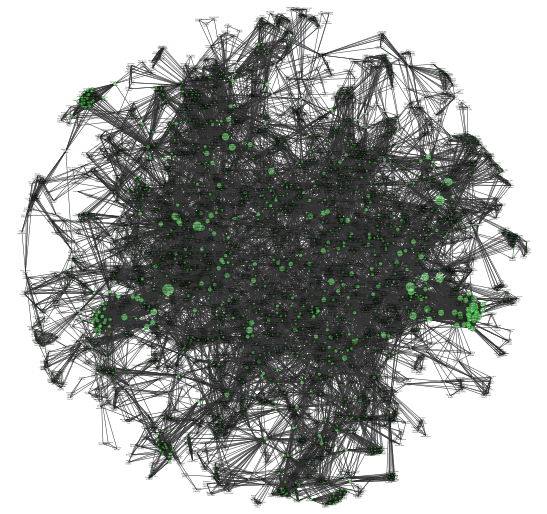
\includegraphics[scale=0.5]{images/Fosiss_GC_final.png}
\caption{Bioemdical research collaboration network (FOSISS) giant component.}\label{Fosiss_GC}
\end{figure}

\FloatBarrier

Other results to report are those of the dynamics of different
variables as the carrying capacity $\nu$ changes. The  most salient
result is that for $\nu$ between $0.19$ and $0.24$, there is an
apparent phase transition in all different topologies and for all the
different variables. Nevertheless, it is worth noticing that the shape
of the phase transition is different according to the topology of the
network at stake. When $\nu$ is between $0.0$ and $0.2$, that is, when there is
no space or a very short one for suspiciousness, all agents cooperate, when
\textit{carrying capacity} is above $0.25$, all agents defect. \textit{Utility},
\textit{strength of interactions}, and \textit{changing state population}
replicate that same behavior for the same limits. \\ 

In \textbf{Figure 2}, we present how the number of cooperators in the population
change as $\nu$ changes. In the Erd\"{o}s-Reny\'i, network, between $0$ and
$0.18$ approximately, all agents converge to a cooperative behavior, from $18$
to $20$, convergence to cooperative state takes longer but eventually all agents
are cooperating. Close to $\nu \approx 0.21$ there is a sharp fall to a point in
which around half the population is cooperating and the rest is
defecting. Reaching $\nu \approx 0.25$ there is another sharp fall of
cooperators and all agents turn into a defecting state.\\


In the case of the Watts-Strogatz, small-world network, the whole population
remains cooperating for ranges between $0$ and $0.2$ but as it gets closer to
$0.2$, more time is needed for the population to become full of cooperators. In
$\nu \approx 0.2$ the cooperators will represent only half of the population and
such number of them will be constant up to $\nu \approx 0.25$ forming a short
plateau. From $\nu \approx 0.25$ to $\nu \approx 0.6$ cooperators will be
present at the beginning of the simulation but will go diminishing as time goes on.
In the case of the Barab\'asi-Albert network, crossing the threshold of $\nu
\approx 0.2$, there is a sharp decrease in the number of cooperators, but stays
constant over time. Such behavior is present for a very short range of $\nu$, and
before $\nu \approx 0.24$, cooperators disappear for the rest of values of
$\nu$. Finally, FOSISS network behaves similar to the other networks in that
there is a fall in the number of cooperators close  $\nu \approx 0.2$. Different
to the other networks, FOSISS network lacks the sharp reduction of
cooperators, instead this population declines smoothly and progressively;
specially, when it reaches a $\nu \approx 0.25$ cooperators go 
decreasing in a less dramatic manner all the way to $\nu \approx 0.5$. It is
also noteworthy that from $\nu = 0$ to $\nu \approx 0.5$ the number of
cooperators converge to a certain amount and stays constant for the rest of the
simulation. 




\begin{figure} [h!]
\centering
\begin{tabular}{cc}
  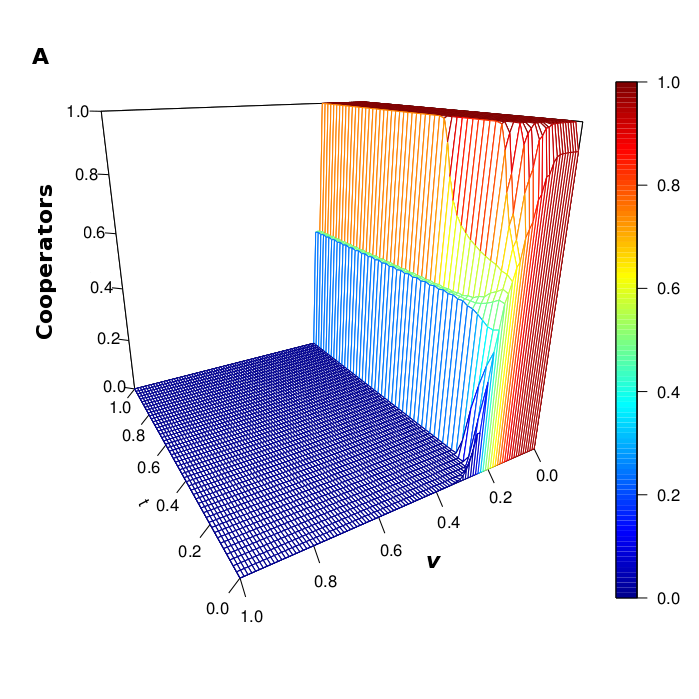
\includegraphics[scale=0.28]{images/erdos_dc_nus_1.png} & 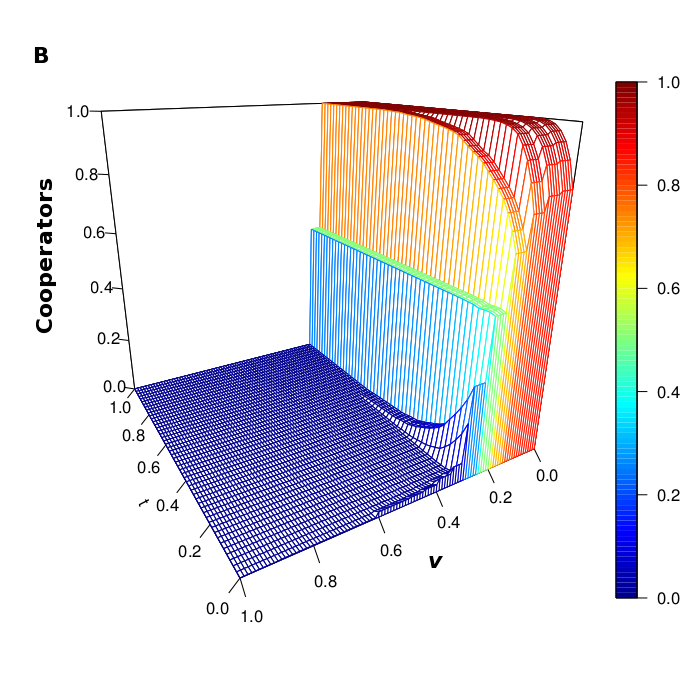
\includegraphics[scale=0.28]{images/watts_dc_nus_1.png}
  \\
  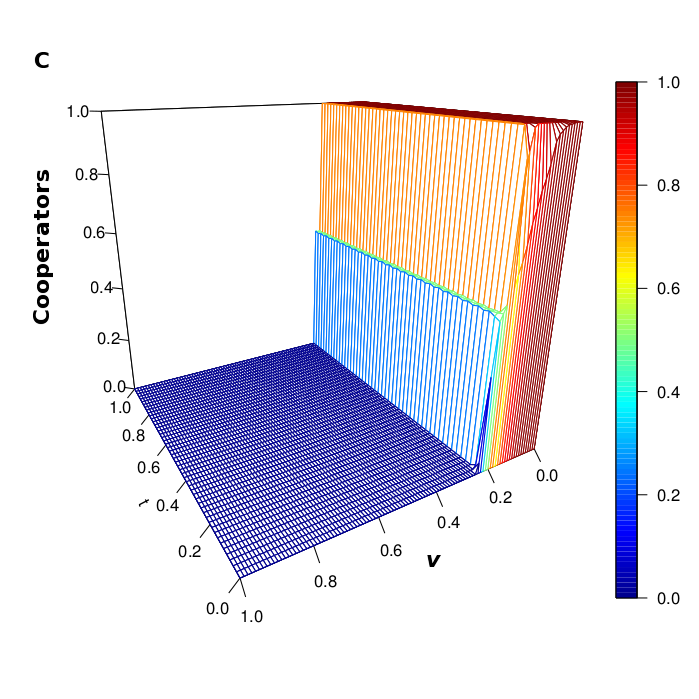
\includegraphics[scale=0.28]{images/barabasi_dc_nus_1.png} & 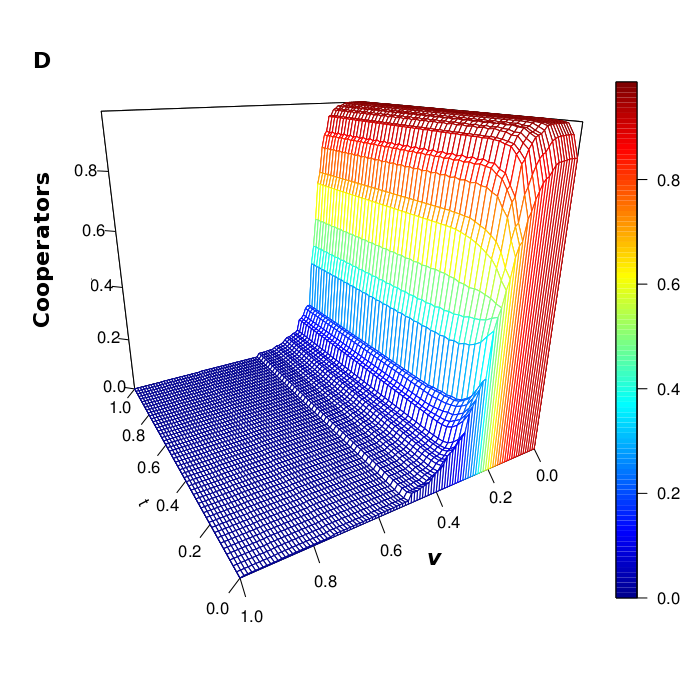
\includegraphics[scale=0.28]{images/fosiss_dc_nus_1.png}
\end{tabular}
\caption{Proportion of cooperators as a function of carrying capacity and time.}\label{CD}
\end{figure}

\FloatBarrier

Utility and strength of interactions dynamics under different $\nu$ emulate the
phase transition found before. In \textbf{Figures 3 and 4}, it can be observed
that there is a drop in utility and strength of interactions according to the
drop in the number of cooperators. Erd\"{o}s-Reny\'i and Barab\'asi-Albert
networks are quite similar in the way these variables fall in two steps, the
first one at $\nu \approx 0.2$ and the next one at $\nu \approx 0.23$. The fall
is sharper still in the Barab\'asi-Albert topology. Utility and strength of
interactions phase transition in Watts-Strogatz network is significantly more
staggered compared to the former networks. In the case of utility, there is a
region in the limits of $\nu \approx 0.25$ and $\nu \approx 0.3$, before utility
goes to $0$, in which it remains low but stable over time. In general, strength
of interactions follows the same pattern as utility but in the same $\nu \approx
0.25$ and $\nu \approx 0.3$, strength of interactions grows to a value that is
higher than the one given by default but soon starts to decrease as the
simulation runs. For FOSISS network, utility and strength of interactions fall
is quite steep but smooth, without sharp cuts. Between $\nu \approx 0.23$ and
$\nu \approx 0.28$, utility and strength of interactions start at their lowest,
but there is a slight increase in both of them.


\begin{figure} [h!]
\centering
\begin{tabular}{cc}

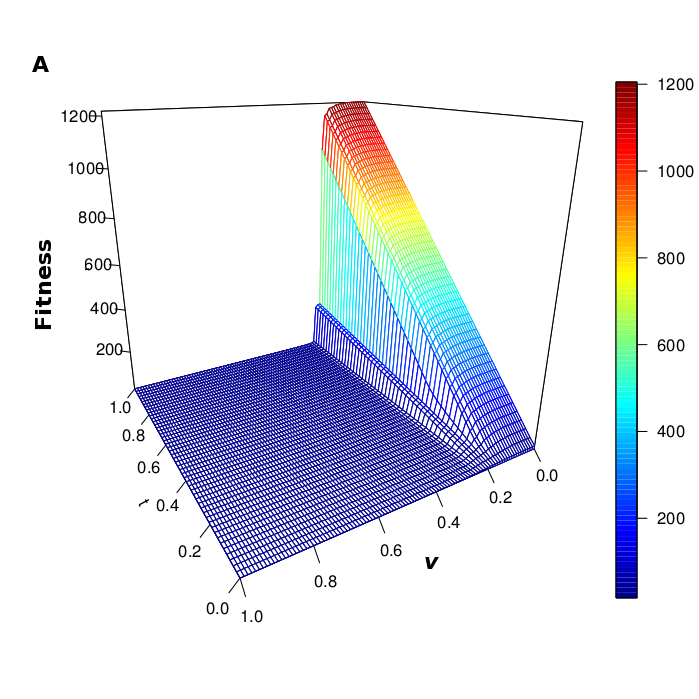
\includegraphics[scale=0.28]{images/erdos_fitness_nus_1.png} & 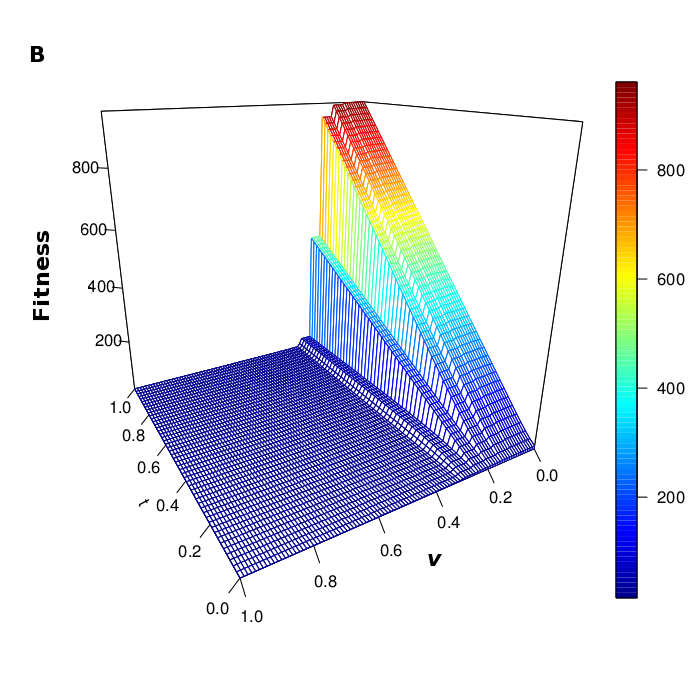
\includegraphics[scale=0.28]{watts_fitness_nus_1.png} \\
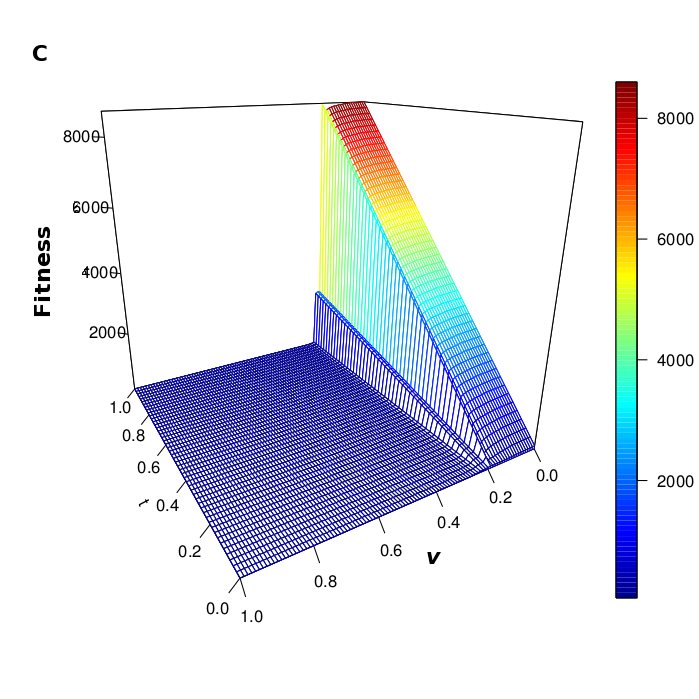
\includegraphics[scale=0.28]{images/barabasi_fitness_nus_1.png} & 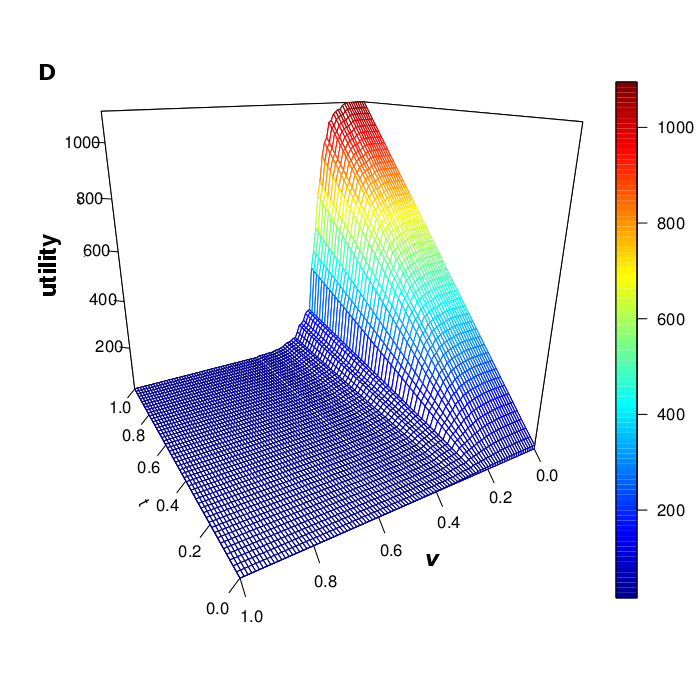
\includegraphics[scale=0.28]{fosiss_fitness_nus_1.png}
\end{tabular}
\caption{Utility $U$ dynamics as a function of carrying capacity $\nu$ and time.}\label{fitness}
\end{figure}

\FloatBarrier


\begin{figure} [h!]
\centering
\begin{tabular}{cc}

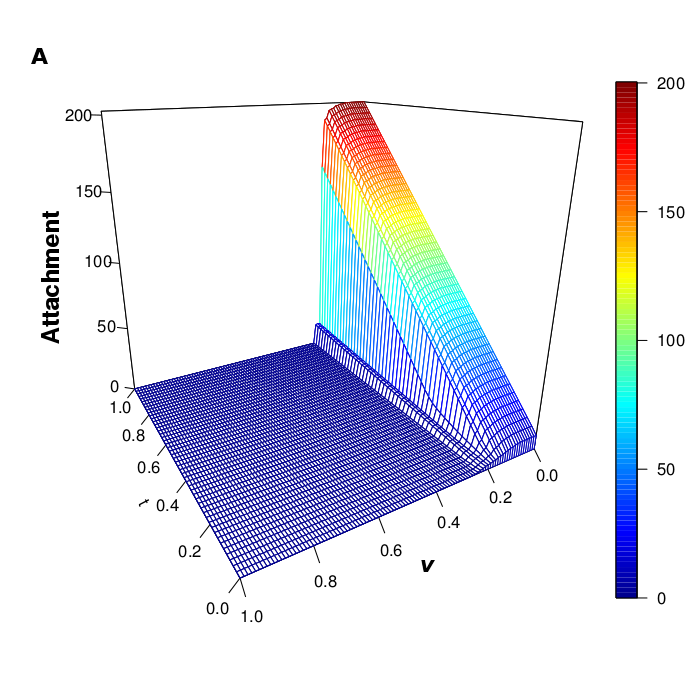
\includegraphics[scale=0.28]{images/erdos_trust_nus_1.png} & 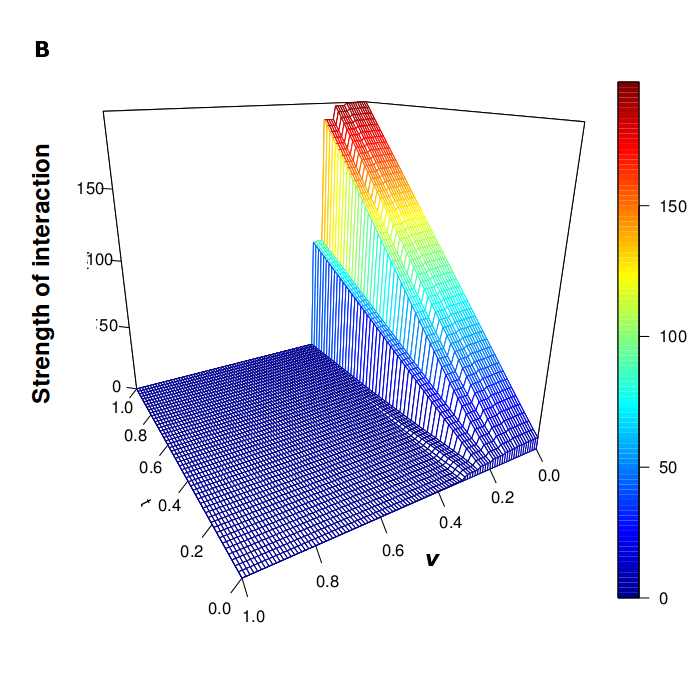
\includegraphics[scale=0.28]{watts_trust_nus_1.png} \\
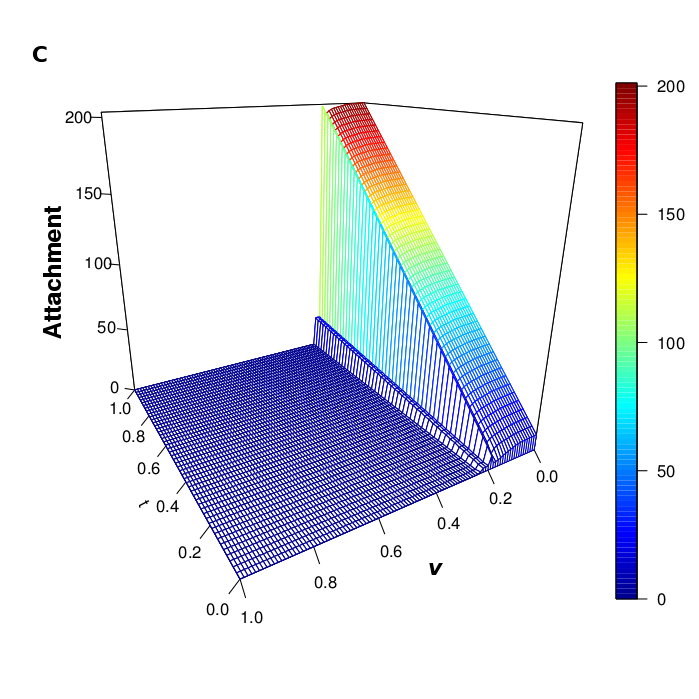
\includegraphics[scale=0.28]{images/barabasi_trust_nus_1.png} & 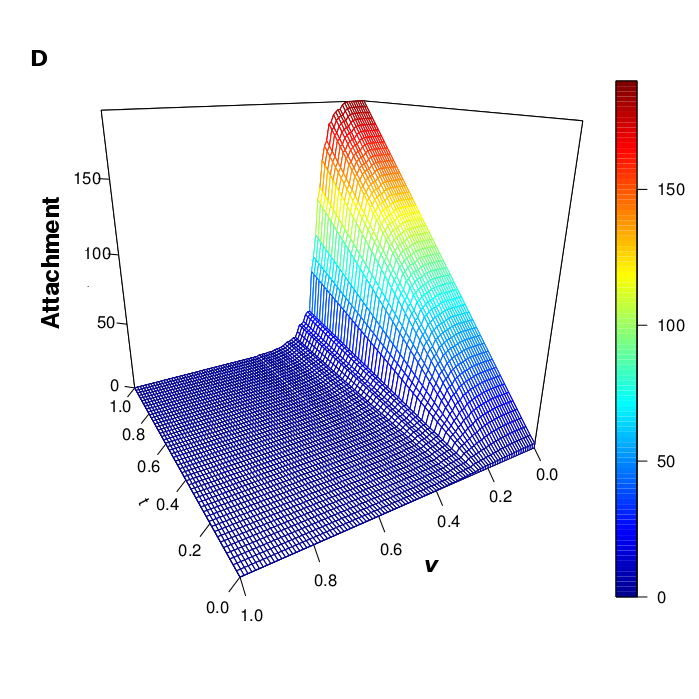
\includegraphics[scale=0.28]{fosiss_trust_nus_1.png}
\end{tabular}
\caption{Strength of interactions $w$ dynamics as a function of carrying capacity $\nu$ and time.}\label{trust}
\end{figure}

\FloatBarrier

We also measured the number of agents shifting states --between cooperating and
defecting- under different $\nu$ values. We found that for all networks there is
a critical point around  $\nu \approx 0.2$ in which all agents are shifting
states. For Erd\"{o}s-Reny\'i and Barab\'asi-Albert networks, for this region,
agents never settle to a single state. Contrary to the former cases, the number
of shifting agents decreases considerably for the Watts-Strogatz and FOSISS
networks, and find an equilibrium state. Once the the limits of this region are
crossed as $\nu$ increases, the number of agents shifting states falls to $0$
and all nodes become defectors. 


\begin{figure} [h!]
\centering
\begin{tabular}{cc}

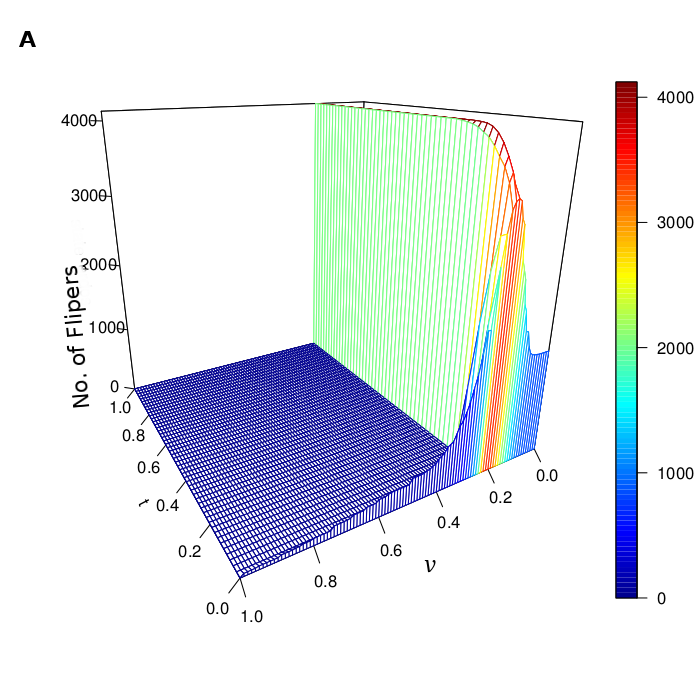
\includegraphics[scale=0.28]{images/erdos_state_nus.png} & 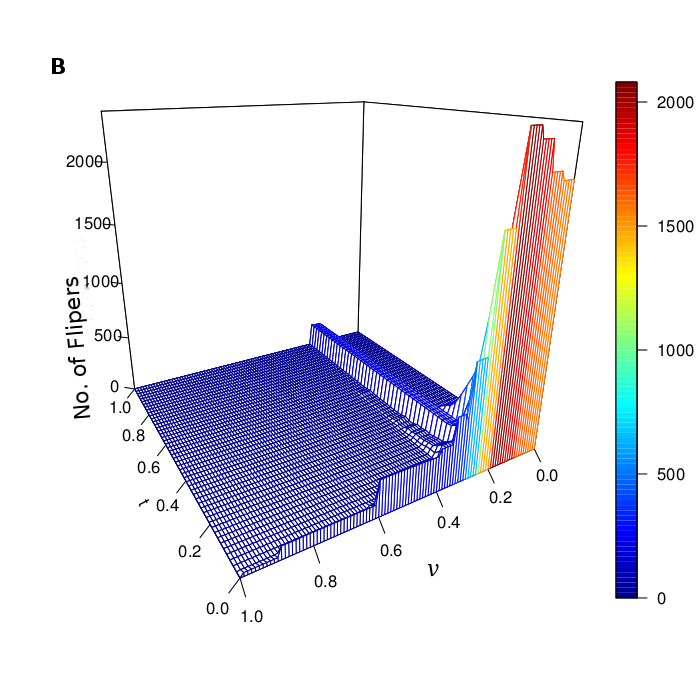
\includegraphics[scale=0.28]{watts_state_nus.png} \\
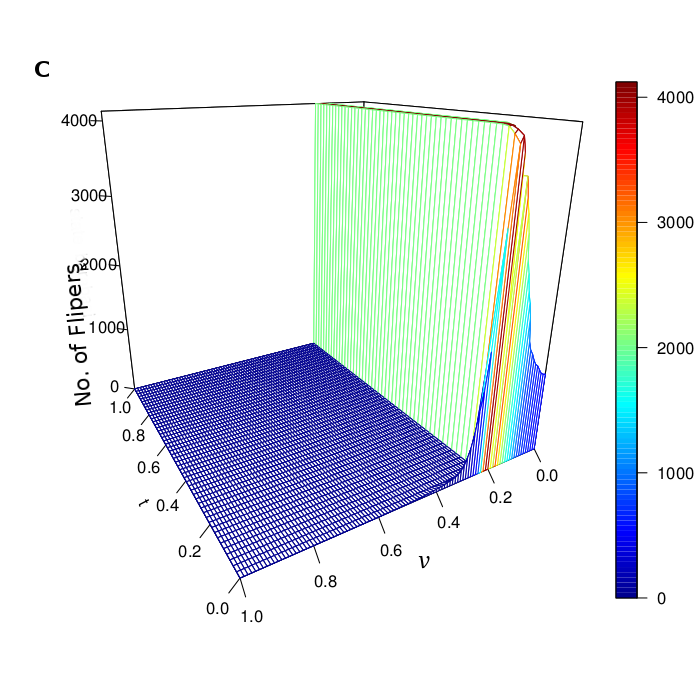
\includegraphics[scale=0.28]{images/barabasi_state_nus.png} & 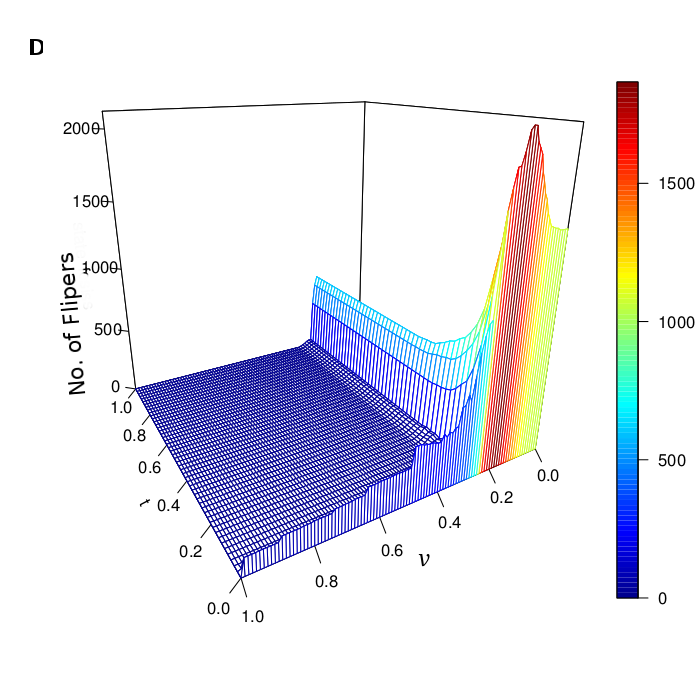
\includegraphics[scale=0.28]{fosiss_state_nus.png}
\end{tabular}
\caption{Shifting population between cooperators and defectors as a function of
  carrying capacity $\nu$ and time.}\label{state} 
\end{figure}

\FloatBarrier

Central to our argument is the differences in utility and strength of
interactions distribution at the end of the simulation, for every topology. We
found that utility distribution for the \textit{FOSISS} network, resembles quite
accurately to the distribution of utility in the Barab\'asi-Albert
network.\\ 


The distribution of utility on each topology is induced by the degree
distribution. This is so, since a given agent (node) will interact with its
neighbors to either cooperate or defect, in such a way that connectivity
influences the number of events played and thus the likelihood of increasing its
corresponding utility. For instance, utility distribution in the random,
Erd\"{o}s-R\'enyi network displays a normal-like curve. The algorithm that
generates this kind of topology, assigns to every node the same probability of
connecting with any other node, which produces a \textit{poissonian} degree
distribution \cite{Erdos1959}. Since the Watts-Strogatz degree distribution is
described by a function that is midways between a random distribution and a
scale-free network \cite{Barrat2000} one may expect also  an intermediate
behavior of the utility distribution. This assumption seems to be fulfilled by
the distribution in Figure 6B. 

The resemblance of the degree-distribution and utility distribution also holds
for the Bar\'abasi-Albert network. As mentioned in the methods section, the
degree distribution of a Bar\'abasi-Albert topology follows a power-law that
describes the fact that there are a small number of nodes with large $k$ and most
nodes have a small $k$ \cite{Barabasi1999}. As it is shown in the following
figure, most utility is concentrated in a few number of agents, while most
agents have a small amount of it. This is consistent with other research in
which concentration of resources, fame or citations in science decreases as a
power-law \cite{Simon1955,Price1965,Merton1968}. FOSISS network utility
distribution is also skewed to the left, similar to that of the
Barab\'asi-Albert network. \\ 


\begin{figure} [h!]
\centering
\begin{tabular}{cc}

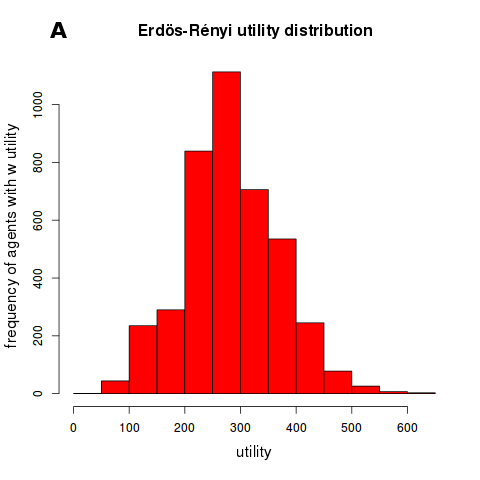
\includegraphics[scale=0.28]{images/erdos_fitness.png} & 
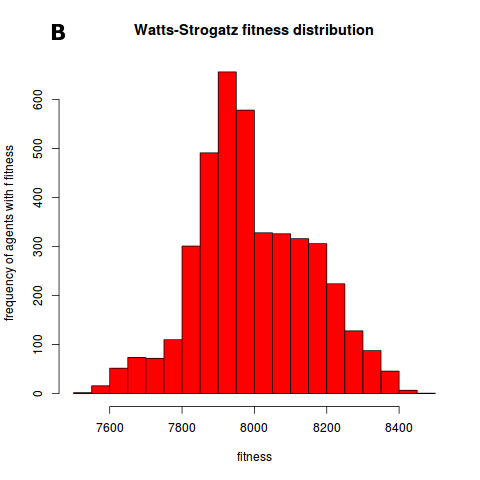
\includegraphics[scale=0.28]{images/watts_fitness.png} \\
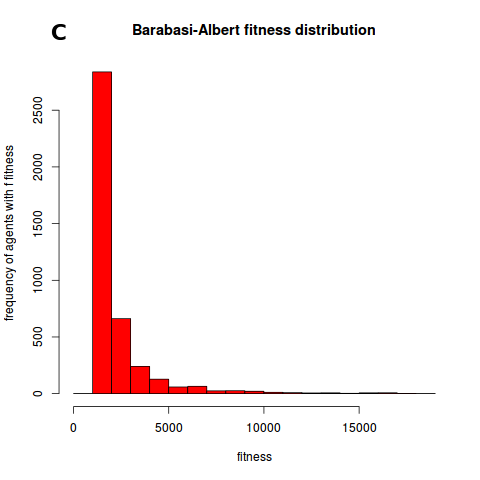
\includegraphics[scale=0.28]{images/barabasi_fitness.png} & 
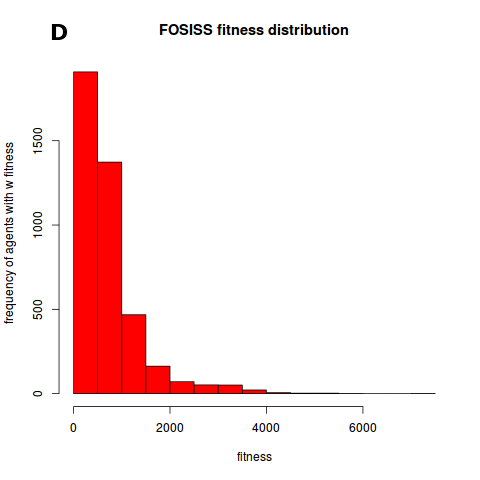
\includegraphics[scale=0.28]{images/fosiss_fitness.png}
\end{tabular}
\caption{Utility distribution on different topologies. A. Random,
  Erd\"{o}s-R\'enyi network displays a normal-like
  distribution. B. Watts-Strogatz network utility distribution is highly skewed
  to the right. C. Barab\'asi-Albert network. Utility is distributed highly
  skewed to the left. D. FOSISS, biomedical researchers collaboration network
  distribution of utility resembles to Barab\'asi-Albert
  network.}\label{histo_fitness} 
\end{figure}

\FloatBarrier

Regarding strength of interactions distribution, the Erd\"{o}s-R\'enyi random
network displays a normal distribution of strength of interactions, as
expected. Again strength of interactions values are highly influenced by the
corresponding degree distribution (Figure 7A). However, in the Watts-Strogatz
network topology (Figure 7B), the strength of interactions distribution is a
highly asymmetric bimodal, with a really-low frequency mode of low strength of
interactions and a highly probability mode for high strength of interactions. A
possible explanation for this phenomenon is that under network topologies
maximizing inter-node communication (by minimizing the average distance between
nodes) such as the Watts-Strogatz, strength of interactions is favored both
among the cooperators (constituting the majority of players) and the
defectors. \\ 


The Barab\'asi-Albert network (7C) presents also a symmetric unimodal
distribution with values higher (on average) than those of the Erd\"{o}s-R\'enyi
random network, this may be the effect of increased communication due to more
efficient network navigability. Interestingly, the network corresponding to the
real FOSISS collaborations (7D) is an asymmetric unimodal distribution in which
moderate to high values of strength of interactions are more likely. We 
hypothesize that this effect is also due to the communication properties of the
network. 

\begin{figure} [h!]
\centering
\begin{tabular}{cc}

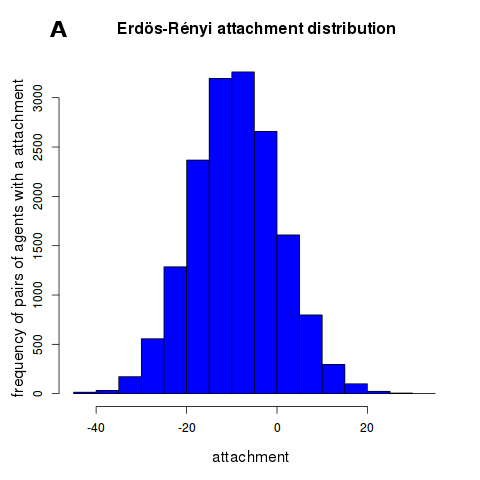
\includegraphics[scale=0.28]{images/erdos_trust.png} & 
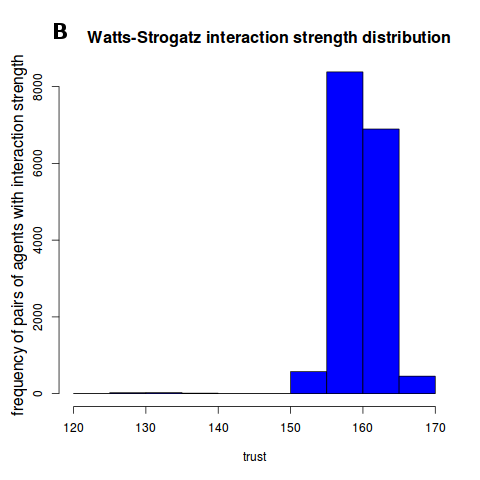
\includegraphics[scale=0.28]{images/watts_trust.png} \\
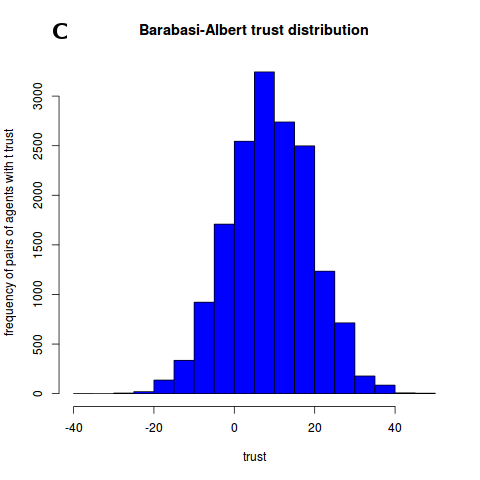
\includegraphics[scale=0.28]{images/barabasi_trust.png} & 
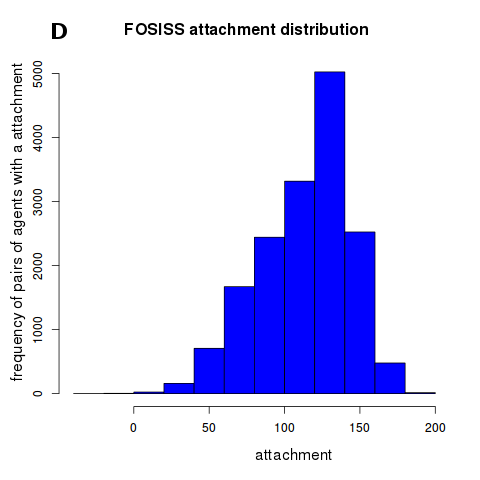
\includegraphics[scale=0.28]{images/fosiss_trust.png}
\end{tabular}
\caption{Strength of interactions distribution on different topologies. A. Random, Erd\"{o}s-R\'enyi network displays a normal-like
  distribution. B. Watts-Strogatz network strength of interactions distribution is bimodal and highly skewed to the right. C.
  Barab\'asi-Albert network strength of interactions distribution is also a normal-like curve. D. FOSISS, biomedical researchers
  collaboration network distribution of strength of interactions is skewed to
  the right.}\label{histo_trust}  
\end{figure}

\FloatBarrier

An interesting feature of highly communicated networks (characterized by high values of clustering coefficient) is the
fact that certainty among players seems to be enhanced, that is, in such networks the rate of change of strategy is
significantly lower (and smoother) than in poorly connected networks. This is another instance in which easier
communication (i.e. lower average minimum path lengths) lead to better performance of the whole collaborative research
system.\\ 


\section{Discussion and Conclusions}
\label{sec:3}

{\color{red}In this work we have analyzed the influence of parameters given by the underlying social structure of a science
collaborative network on collective strength of interactions and utility dynamical behavior, based on a class of iterated
PD and coordination games. Such parameters include mainly local and global connectivity like the degree centrality and
average clustering coefficient, as well as communication patterns.}\\

{\color{red}Under the assumptions given by the model, we were able to notice
  that, in general, communication within the social
collaborative networks has a positive correlation with average strength of interactions between the individuals partaking in the games and
also with the global collective utility (given by the sum of the individual payoffs). The better the
communication among players, the higher the strength of interactions and the utility leading to an optimized functioning of the whole
\emph{scientific collaboration system}. This is an important result that may be useful for scientific policy planning
and may set a foundation for the optimal use of social networks in scientific collaboration as a means to improve the
relationships among collaborating peers and thus ultimately the performance of research systems. 
We obviously need more qualitative work in order to validate these results from a sociological and anthropological
perspective.\\ %Furthermore, such validation is necessary because, as we said at
             %the beginning of this work, \emph{strength of interactions} can
             %have many different meanings and implementations in the real
             %world. The same we can say about \emph{utility} and most of all,
             %about the very idea of the game we explored here since ``playing
             %the game'' must have so, many different meanings among resarchers
             %and their communities.}\\ 

{\color{red}To close this article, we would like to comment on three issues we consider important. The first one is about
confronting our results with data available to us from the biomedical research community. Second, some remarks we believe are important
about the role of computational simulations in the social sciences. Finally we would like to comment on our
future work.}\\


{\color{red}The two main results of our model are the smoothness in the phase transition-like behavior for different parameters and the distribution of utility and strength of interactions in the FOSISS network compared to other networks and their topologies. We are certain that the particular structure of FOSISS network is playing a central role in the results and because of that we would like to discuss it a little bit further.}\\

{\color{red}FOSISS network is higly hierarchical according to its heterogeneity of $0.873$. Because of it, one would
  expect to find the presence of important hubs \cite{Wu-etal2008}, that is, a few researchers control the whole
  network, as has been reported in some other places \cite{yousefi-etal2008}. Surprisingly, FOSISS network
  centralization is very low $0.023$, i.e. there are no researchers that centralize the majority of connections. Our
  guess is that the network is composed of many small communities or groups with a central researcher or Principal
  Investigator (PI). If this is the case in the FOSISS network, it means that those groups have a very hierarchic structure as well.}\\

{\color{red}Under such structure, when the clustering coefficient is considered, it can be said that groups are also well connected
but that inter-group connections are sparse. In other words, individual groups are strongly connected but the network
as a whole is supported by a small number of links. We came by this idea partially from
another study about scientific collaborations based on co-authorships in one of
the research centers that is part 
of the FOSISS network \cite{HernandezLemus2013}. In the cited reference an apparently well integrated community was
found (high clustering coefficient and a very short characteristic path length). Such integration was mostly
superficial, since it depended on the presence of external collaborators from other research institutions (most of them from overseas). 
Removing these external collaborators broke down the network into small subgraphs that worked independently. Remarkably those subgraphs corresponded to the real
groups of that research center.  What is more, several groups had a hierarchical structure as 
the one we suspect is common in FOSISS subgraphs. The results showed that collaboration was poor between groups but strong
among the members of each group, and that collaboration among groups doesn't emerge bottom-up, instead it seems to be promoted from the
top, from the administrative authorities.}\\ 

{\color{red}We believe that the the situation just refered is also true for the whole biomedical research community in M\'exico. The
amount of PIs who have also been collaborators in other projects is about one fifth of the total number of participants.
This is a number big enough to connect the whole network in one giant component. Yet, due to the topological
characteristics of the FOSISS network, it appears to be the case that researchers can be the leaders in one project and
collaborators of different project of \emph{its own research group}. CONACyT's funding policies makes it impossible for a
researcher to get a grant from a fund if that researcher has an ongoing project with a grant from that same fund. That
is, a researcher can ask for a grant from FOSISS if and only if at the moment he
doesn't have a grant from FOSISS already. This
policy has lead researchers from the same group to ask for grants from the same fund in order to rise their
budgets. A consequence of this behavior is that group interactions get reinforced, but integroup connections not necessarily so.}\\

{\color{red}As is common among scientific communities in biomedical research, PIs play a central role in the network. Strong PIs and
well connected groups seem to be somehow responsible for the high levels of strength of interactions and the centralization of utility in
our simulation. As for what seems to be phase transitions, in the case of FOSISS networks, these are smoother than
those in the other networks with different topologies, even for those with a small-world topology. We think that this
behavior is also the result of the hierarchical structure already mentioned. If this is true, strength of interactions is first lost in the
edges that link diffrent goups and then in the edges that connect members of the groups. Connections between groups would not
be as dense as those inside the groups, which means that there would not be enough information of the behavior of one group regarding
its neighbors to constrain them as it seems to happen with individual researchers inside their communities. Nevertheless,
if values of the carrying capacity $\nu$ keep increasing and it becomes more
difficult to strengthen interactions, then strength of interactions begins to diminish inside groups.}\\

{\color{red}Another issue that we would like to mention about FOSISS network topology is that it is not a robust collaboration network.
At the level of groups, these might be well connected and consolidated but at the level of the network, this could be
no more than an aggregate of individual groups. A robust network would be resistant to changes in the connections
between groups but in the case of FOSISS, it seems that the network would brake down into
small research groups by cutting some edges, as it happened in our co-authorship
collaboration network \cite{HernandezLemus2013}. The lack of robustness might be 
indicative of the fact that resources stay inside the groups, that is, they do not circulate through or articulate different communities. For
example, one may think of certain expensive technologies for genomic research that could be bought once and shared
among research groups, however, this doesn't seem to happen very often. There are some other
consequences, such as low communication among groups, atomization of practices and know-hows, redundancy in equipment tenancy,
difficulties for implementing community-wide infrastructures such as biobanks, etc.}\\ 

%% {\color{red}Regarding simulations and social science. We believe that social scientists may learn many lessons from
%%   computational modeling. Tipically, the use of computational modeling as part of the social sciences
%%   has been justified by arguing that such methods allow to understand the connection between the level of the individual
%%   and the level of the group, they make possible to explore different outcomes by tuning different parameters and to
%%   perform --virtual-- experiementation, as well as studying different propensities as Stephen Lansing calls them
%%   \cite{Epstein1996,Lansing2002}. All these are important arguments but we would also like to say something else about 
%%   them. When presenting computational modeling to non-computational social scientists (specially anthropologists) one gets
%%   confronted with several critiques from which, the most common are that computational modeling tends to ignore cultural
%%   differences (should be noticed that cultural differences is not the same as social differences), and that it is hard to grasp the cultural
%%   meaning or significance of the dynamics expressed in the simulation. Because of this kind of observations we are
%%   particularly interested in not forgiving from our work the ethnographical, culturally loaded content of social life,
%%   while recognizing the value of computational simulations.}\\ 

%% {\color{red}We believe that computational simulations are methodologically valuable for two reasons. The first one is that
%% simulations can play an important role in social research as heuristics. If, as we have been doing in this project, fieldwork
%% observations influence and inspire the development of a computational simulation, parameters must be an abstraction of
%% those observations or at least of part of them. In this sense, the outcomes of simulations are a guide towards new
%% questions and future fieldwork explorations at the time that it constrains and helps to prioritize what is to be
%% observed. For example, from out results it seems mandatory to interview different research groups in order to disclose
%% internal group dynamics and how and which are the terms for collaboration between groups. The second reason emerges from
%% the first, we think that simulations are excellent hypothesis generators for the social sciences. Due to the
%% imposibility of ``observing'' the social dynamics on real-time, just because we can only observe locally while one is
%% doing fieldwork, there are left a few options to see how local dynamics may produce emergent patterns. Simulations may
%% be of great help to elaborate guesses about the mechanisms for the behaviors observed at the local scale, as well as for
%% the global. For example, we could guess that the hierarchical structure without hubs imposes strong limits to the flow
%% of resources and information or that we can expect certain cultural intepretation regarding collaboration due to the
%% position of researchers in the network. Such hypothesis can be computationally tested too.}\\

{\color{red}On these grounds, part of our future work is based on some of the results presented here. We would like to
identify researchers in our simulations and corroborate their situation in the model and in the real world. We are
also interested in going back to the field and interviewing those groups with an interesting behavior found in our
simulations, probably we would follow a similar strategy as the one developed in \cite{Haraetal2003}. Finding
communities beyond the level of the groups is an important task. We think that there are many possibilities that emerge
from the integration of different methodologies. Moreover, studying social processes in science is particularly
attractive due to the amounts of data already available that can be easily collected. This is a privilege because
simulations can be designed on real world data, something that only very recently has become possible
\cite{Barabasi2011}.\\


No doubt, social sciences are getting more ``computational''. This can be seen everywhere, but curiously enough,
disciplines like physicis and computer science are the ones who are moving towards the social sciences and not so much
the other way around. It might be the case that the pioneering disciplines in the computational social sciences will set
the agenda, an agenda that will apparently be mostly based on taking advantage of big data and on hypothesis-free approaches. We
believe that the social sciences have important questions that should be added to that agenda and those questions may not
be answered only by big data techniques but they may require creating models and simulations in the style of the best
hypothesis-driven research.} 
 
%Text with citations \cite{RefB} and \cite{RefJ}.
%\subsection{Subsection title}
%\label{sec:2}
%as required. Don't forget to give each section
%and subsection a unique label (see Sect.~\ref{sec:1}).
%\paragraph{Paragraph headings} Use paragraph headings as needed.
%\begin{equation}
%a^2+b^2=c^2
%\end{equation}

% For one-column wide figures use
%\begin{figure}
% Use the relevant command to insert your figure file.
% For example, with the graphicx package use
%  \includegraphics{images/example.eps}
% figure caption is below the figure
%\caption{Please write your figure caption here}
%\label{fig:1}       % Give a unique label
%\end{figure}
%
% For two-column wide figures use
%\begin{figure*}
% Use the relevant command to insert your figure file.
% For example, with the graphicx package use
%  \includegraphics[width=0.75\textwidth]{example.eps}
% figure caption is below the figure
%\caption{Please write your figure caption here}
%\label{fig:2}       % Give a unique label
%\end{figure*}
%
% hello, friend
%
% For tables use
%\begin{table}
% table caption is above the table
%\section{%\caption{Please write your table caption here}}
%\label{tab:1}       % Give a unique label
% For LaTeX tables use
%\begin{tabular}{lll}
%\hline\noalign{\smallskip}
%first & second & third  \\
%\noalign{\smallskip}\hline\noalign{\smallskip}
%number & number & number \\
%number & number & number \\
%\noalign{\smallskip}\hline
%\end{tabular}
%\end{table}


\section{acknowledgements}
The authors gratefully acknowledge support by grants: CB-222220-R/2013 and
CB-179431/2012 (Consejo Nacional de Ciencia y Tecnolog\'ia). We would also like
to acknowledge CONACyT for letting us access their database. Finally, we
acknowledge the help of Francisco Allende for his work curating 
databases of researchers.





%If you'd like to thank anyone, place your comments here
%and remove the percent signs.


% BibTeX users please use one of
%\bibliographystyle{spbasic}      % basic style, author-year citations
%\bibliographystyle{spmpsci}      % mathematics and physical sciences
%\bibliographystyle{spphys}       % APS-like style for physics
%\bibliography{}   % name your BibTeX data base

% Non-BibTeX users please use

\begin{thebibliography}{100}

\bibitem{Vermeulen2013} Vermeulen, Nikki; Parker, John N \& Penders,
  Bart, Understanding life together: A brief history of collaboration
  in biology, \textit{Endeavour}, 37(3): 162-171 (2013) 

\bibitem{KnorrCetina1999} Knorr-Cetina, Karol; \textit{Epistemic
  cultures: how the sciences make knowledge}, MIT Press, Cambridge, MA
  (1999) 

\bibitem{Strasser2006} Strasser, B.J. Collecting and Experimenting:
  The Moral Economies of Biological Research, 1960s-1980s.
  \textit{Preprint no. 310.} Berlin: Max Planck Institute for the
  History of Science, (2006) 

\bibitem{Muller2012} M\"{u}ller-Wille, S. \& Charmantier. I.  Natural
  history and information overload: The case of Linnaeus.
  \textit{Studies in History and Philosophy of Biological and
    Biomedical Sciences.} 43:4-15, (2012) 

\bibitem{Strasser2012} Strasser, BJ. Data-driven sciences: From
  wonder cabinets to electronic databases. \textit{Studies in History
    and Philosophy of Biological and Biomedical Sciences} 43:85-87,
  (2012)

\bibitem{Sonnenwald2007} Sonnenwald, DH. Scientific Collaborations. \textit{Annual Review of Information Science and
  Technology}, 41.

\bibitem{Newman2001} Newman, MEJ. Clustering and preferential
  attachment in growing networks. \textit{Physical Review E},
  64:025102-1/025102-4, (2001) 

\bibitem{Newman2004} Newman, MEJ. Coauthorship networks and patterns
  of scientific collaboration. \textit{PNAS}, 101, no. suppl 1,
  5200-5205 (2004) 

\bibitem{Elango2012} Elango, B. \& Rajendran, J. Authorship Trends and
  Collaboration Pattern in the Marine Sciences Literature: A
  Scientometric Study. \textit{International Journal of Information
    Dissemination and Technology}, 2(3), 166-169, (2012)
  
  
\bibitem{HernandezLemus2013} Hern\'andez-Lemus, Enrique \&
  Siqueiros-Garc\'ia JM, Information theoretical methods for complex
  network structure reconstruction. \textit{Complex Adaptive Systems
    Modeling}. 1: 8, doi:10.1186/2194-3206-1-8 (2013).

\bibitem{Gilbert1997} Gilbert, N. A Simulation of the Structure of
  Academic Science. \textit{Sociological Research Online}, 2(2) 3,
  http://www.socresonline.org.uk/2/2/3.html 
  
\bibitem{Edmonds2011} Edmonds, B., Gilbert, N., Ahrweiler, P., \&
  Scharnhorst, A. Simulating the Social Processes of Science.
  \textit{Journal of Artificial Societies and Social Simulation},
  14(4) 14,  http://www.jasss.soc.surrey.ac.uk/14/4/14.html
  
\bibitem{Hara_etal_2002} Hara, N. Solomon, P. Kim SL. Sonnenwald DH. An Emerging View of Scientific Collaboration:
  Scientists’ Perspectives on Collaboration and Factors that Impact Collaboration. \textit{Journal of the American
    Society for Information Science and Technology}, 54(10):952–965, (2003) 

\bibitem{Lieberman_etal_2005} Lieberman, E. Hauert, C. \& Nowak,
  MA. Evolutionary Dynamics on Graphs. Nature, 433, doi:0.1038/nature03204 (2005).

  
\bibitem{Lo2004} Lo, T.S., Chan, H.Y., Hui, P.M., Johnson, N.F.,
  Theory of networked minority games based on strategy pattern
  dynamics, \textit{Physical Review E} 70, 056012 (2004) 

\bibitem{Buesser2012} Buesser, P. and Tomassini, M., Evolution of
  cooperation on spatially embedded networks, \textit{Physical Review E} 86,
  066107 (2012)  

\bibitem{Ichinose2013} Ichinose, G., Tenguishi, Y., and Tanizawa, T.,
  Robustness of cooperation on scale-free networks under continuous
  topological change, \textit{Physical Review E} 88, 052808 (2013) 

\bibitem{Ahmed2014} Ahmed, A., Karlapalem, K., Inequity aversion and
  the evolution of cooperation, \textit{Physical Review E} 89, 022802, (2014)

\bibitem{Vilone2014} Vilone, D., Ramasco, J.J., S\'anchez, A., San
  Miguel, M., Social imitation versus strategic choice, or consensus
  versus cooperation, in the networked Prisoner’s Dilemma,
  \textit{Physical Review E} 90, 022810, (2014) 
 
\bibitem{Wardil2015} Wardil, L., Hauert, C., Cooperation and coauthorship in
  scientific publishing, Physical Review E 91, 012825, (2015)
 
 \bibitem{hanauske2012} Hanauske, M., Evolutionary Game Theory and Complex Networks of Scientific Information, in A. Scharnhorst et al. (eds.), \textit{Models of Science Dynamics, Understanding Complex Systems Series}, Springer Berlin Heidelberg, (2012)
  
\bibitem{Szabo2007} Szab\'o, Gy\"{o}rgy \& F\'ath, G\'abor,
  Evolutionary games on graphs. \textit{Physics Reports}, 446: 97-216
  (2007) 

\bibitem{Nowak1992} Nowak, Martin A. \& May, Robert M, Evolutionary
  Games and Spatial Chaos. \textit{Nature}, 359: 826-829, (1992)

\bibitem{Nowak2006} Oshtuki, Hisashi, Hauert, Christoph, Lieberman, Erez \& Nowak, Martin A, A simple rule for the evolution of cooperation on social graphs. \textit{Nature}, 441: 502-505 (2006)

\bibitem{Axelrod2006} Axelrod, Robert, \textit{Evolution of cooperation: Revised edition}, Basic Books, Cambridge, MA (2006)

\bibitem{Nowak2011} Nowak, Martin A. \& Highfield, Roger,
  \textit{Supercooperators. Altruism, Evolution, and Why We Need Each
    Other to Succeed}. Free Press, New York, NY  (2011)

\bibitem{Santos2006} Santos, Francisco C., Pacheco, Jorge M., Lenaerts, Tom, Cooperation prevails when individuals adjust their social ties. \textit{PLoS Computational Biology}. 2(10): 1284-1291 (2006)

\bibitem{Santos2005} Santos, F.C. \& Pacheco, J.M., Scale-Free
  Networks Provide a Unifying Framework for the Emergence of
  Cooperation. \textit{PRL}, 95: 098104-1 to 098104-4, (2005) 

\bibitem{Hauert2004} Hauert, Christoph \& Doebeli, Michael, Spatial
  structure often inhibits the evolution of cooperation in the
  snowdrift game. \textit{Nature}, 428: 643-646,  (2004)

\bibitem{Erdos1959} Erd\"{o}s, P. \& Reny\'i, A. On Random Graphs. \textit{Publ. Math}, 6:290 (1959).

\bibitem{Watts1998} Watts, Duncan J. \& Strogatz, Steven H, Collective dynamics
  of 'small-world' networks. \textit{Nature}, 393: 440-442 (1998)
  
  \bibitem{Barrat2000} Barrat, A.; Weigt, M., On the properties of small-world network models, \textit{European Physical Journal B} 13 (3): 547–560, (2000)

\bibitem{Barabasi1999} Barab\'asi, Albert-L\'aszl\'o. \& Albert, R\'eka, Emergence of Scaling in Random Networks. \textit{Science}, 286: 509-512 (1999)
  
\bibitem{Shannon2003} Shannon P, Markiel A, Ozier O, Baliga NS, Wang JT, Ramage D, Amin N, Schwikowski B, Ideker T. Cytoscape: a software environment for integrated models of biomolecular interaction networks. \textit{Genome Research}, 13(11):2498-504, (2003)

\bibitem{Wu-etal2008}Jun Wu, Yue-Jin Tan, Hong-Zhong Deng, Da-Zhi Zhu. A new measure of heterogeneity of complex networks based on degree sequence.  Eds. Ali Minai, Dan Braha, Yaneer Bar-Yam  \emph{Unifying Themes in Complex Systems. Proceedings of the Sixth International Conference on Complex Systems}, Springer Berlin Heidelberg, 66-73, (2008)
  
\bibitem{yousefi-etal2008} Yousefi-Nooraie R, Akbari-Kamrani M, Hanneman RA, Etemadi A. Association between co-authorship network and scientific productivity and impact indicators in academic medical research centers: A case study in Iran. \textit{Health Research Policy and Systems} 6:9 (2008) doi:10.1186/1478-4505-6-9.
  
%%Discusion references


\bibitem{Simon1955} Simon, HA. On a class of skew distribution functions. \textit{Biometrika}, 42 (3-4): 425-440, (1955)

\bibitem{Price1965} Price, Derek JS. Networks of Scientific Papers. \textit{Science}, 149(3683): 510-515, (1965)

\bibitem{Merton1968} Merton, Robert K, The Matthew Effect in Science, \textit{Science}, 159(3810): 56-63 (1968)

\bibitem{Epstein1996} Epstein JM \& Axtell R. \textit{Growing artificial societies. Social science from the bottom up}. The
  Brookings Institution Press and The MIT Press, Washington, DC. (1996)

\bibitem{Lansing2002} Lansing JS. ``Artificial Societies'' and the Social
  Sciences. \textit{Artificial Life}, 8:279-292, (2002)

\bibitem{Haraetal2003} Hara N, Solomon P, Kim SL, Sonnenwald DH. An emerging
  view of scientific collaboration: Scientists' perspectives on collaboration
  and factors that impact collaboration. Journal of the American Society for
  Information Science and Technology, 54(10):952–965, 2003
   

\bibitem{Barabasi2011} Barab\'asi, AL. The network takeover. \textit{Nature}, 8:14–16, (2012)

\bibitem{Conteetal2012} Conte R, Gilbert N, Bonelli G, Cioffi-Revilla C,
  Deffuant G, Kertesz J, Loreto V, Moat S, Nadal J.-P,  Sanchez A, Nowak A,
  Flache  A, San Miguel M, Helbing D. Manifesto of computational social
  science. \textit{The European Physical Journal, Special Topics} 214(1):325–346, (2012) 
  
  %
% and use \bibitem to create references. Consult the Instructions
% for authors for reference list style.
%
%\bibitem{RefJ}
% Format for Journal Reference
%Author, Article title, Journal, Volume, page numbers (year)
% Format for books
%\bibitem{RefB}
%Author, Book title, page numbers. Publisher, place (year)
% etc
\end{thebibliography}

\end{document}
% end of file template.tex
